\subsection{MUMPS: Process Pinning}
\label{subseq:mm-mumps-process-pinning}

Due to intensive and complex manipulations with frontal and contribution matrices, one can assume that MUMPS belongs to a group of memory bound applications. In this case, memory access becomes a bottleneck. A common way to improve performance of a memory bound computer program running on distributed-memory machines is to distribute MPI processes equally among all available NUMA domains within a compute node. Given the fact that each NUMA domain possesses its own system bus, this strategy allows to reduce conjunction of memory traffic by balancing data requests equally among the memory channels.\\


However, due to the fact that MUMPS uses both task and data parallelism as well as a complex, static and dynamic, task scheduling, it becomes difficult to state which process pinning strategy is better to use i.e. \textit{close} or \textit{spread}, described in chapter \ref{subseq:matrix-sets-and-hardware}.\\


Therefore, a couple of tests were carried out with both GRS and SuiteSparse matrix sets in order to investigate influence of different pinning strategies on MUMPS parallel performance. For this group of tests, MUMPS was ran with the default settings but with a specific fill-in reducing algorithm assigned for each test-case according to tables \ref{table:GRS-ordering-assignment} and \ref{table:SuiteSparse-ordering-assignment}. The tests were performed on both HW1 and HW2 machines using only the flat-MPI mode i.e. 1 OpenMP thread per MPI process. Comparison between different hardware also allows to investigate influence of different numbers of independent system buses within a compute-node on parallel performance of MUMPS since HW1 and HW2 machines have 2 and 4 of NUMA domains, respectively. Results are shown in figures \ref{fig:mumps-close-vs-spread-1}, \ref{fig:mumps-close-vs-spread-2}, \ref{fig:mumps-close-vs-spread-3} and in appendix \ref{app:mm-mumps-process-pinning}. The graphs depict the total execution time of MUMPS spent on a test-case i.e. time spent on the analysis, factorization and solution phases.\\

\figpointer{\ref{fig:mumps-close-vs-spread-1}}
\begin{figure}[htpb]
\centering
	\begin{tabular}{cc}
	\subfloat[HW1 - pwr-3d]{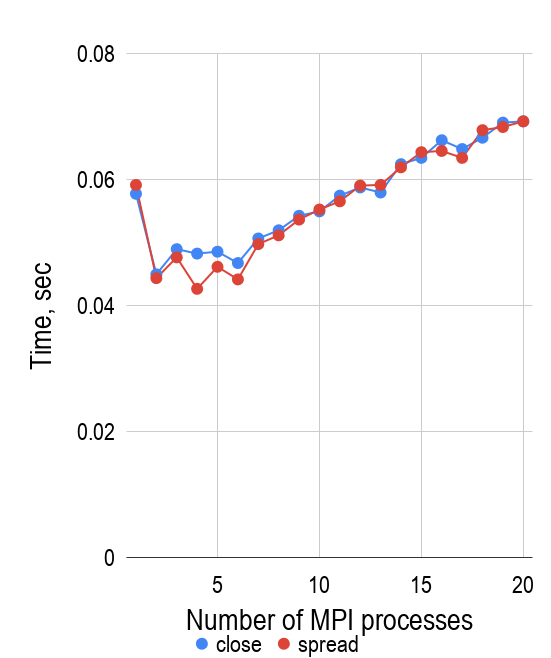
\includegraphics[width=0.48\textwidth]{figures/chapter-2/spread-vs-close/grs-cluster/pwr-3d.png}} &
		\subfloat[HW2 - pwr-3d]{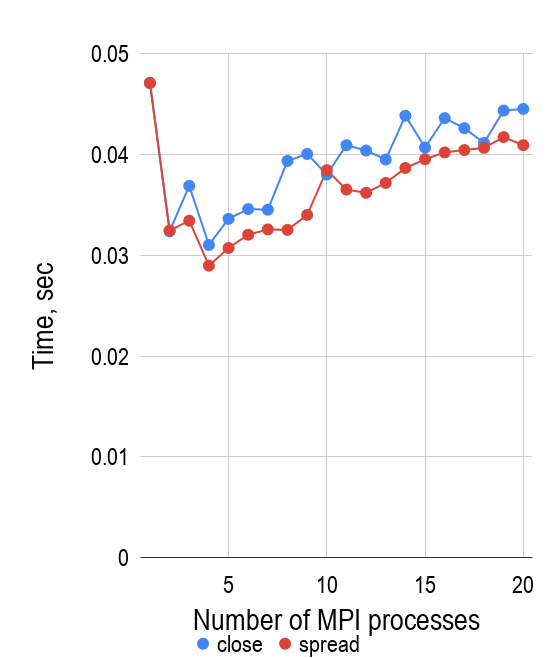
\includegraphics[width=0.48\textwidth]{figures/chapter-2/spread-vs-close/linux-cluster/pwr-3d.png}} \\
		\subfloat[HW1 - cube-64]{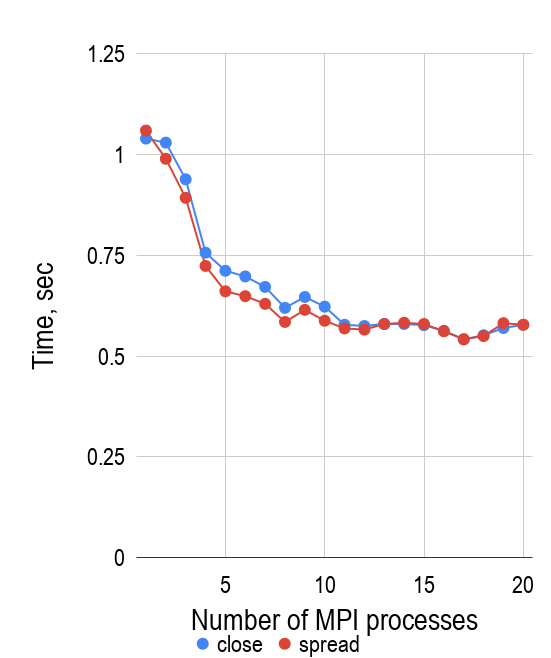
\includegraphics[width=0.48\textwidth]{figures/chapter-2/spread-vs-close/grs-cluster/cube-64.png}} &
		\subfloat[HW2 - cube-64]{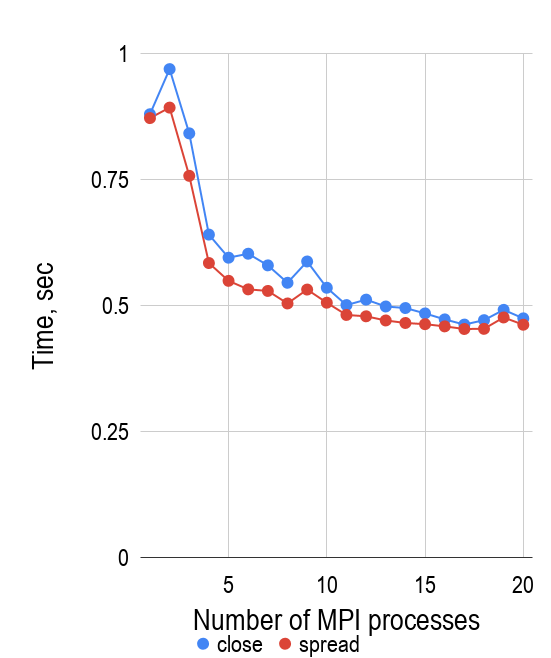
\includegraphics[width=0.48\textwidth]{figures/chapter-2/spread-vs-close/linux-cluster/cube-64.png}} \\
	\end{tabular}
	\caption{Comparison of \textit{close} and \textit{spread} pinning strategies}
	\label{fig:mumps-close-vs-spread-1}
\end{figure}



\figpointer{\ref{fig:mumps-close-vs-spread-2}}
\begin{figure}[htpb]
\centering
	\begin{tabular}{cc}
		\subfloat[HW1 - cube-645]{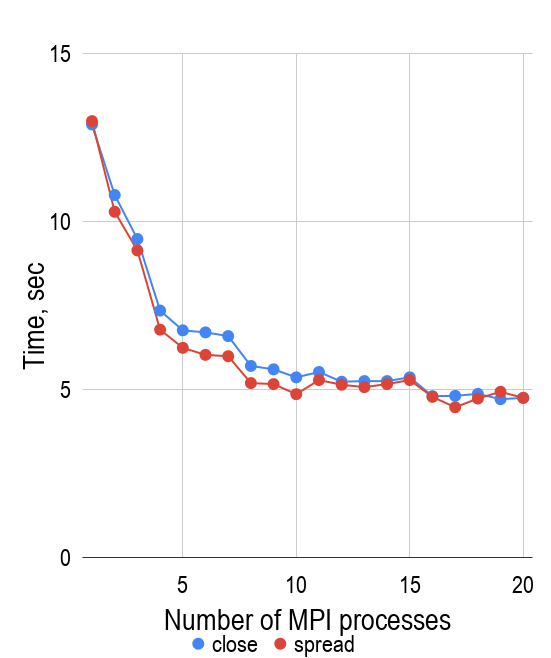
\includegraphics[width=0.48\textwidth]{figures/chapter-2/spread-vs-close/grs-cluster/cube-645.png}} &
		\subfloat[HW2 - cube-645]{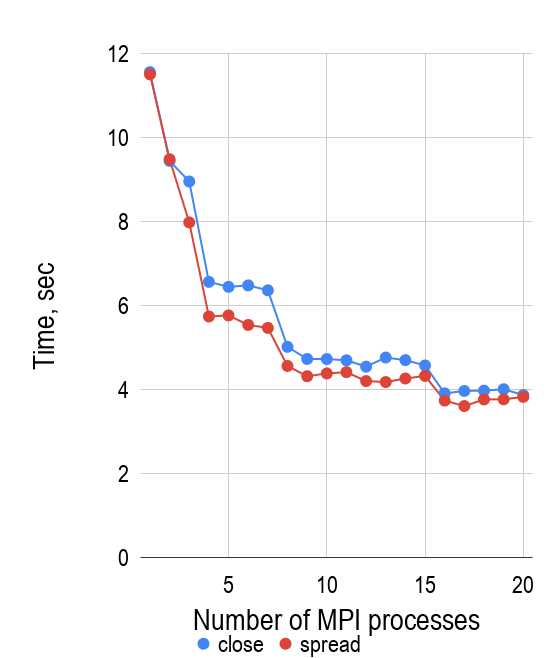
\includegraphics[width=0.48\textwidth]{figures/chapter-2/spread-vs-close/linux-cluster/cube-645.png}} \\
		\subfloat[HW1 - k3-18]{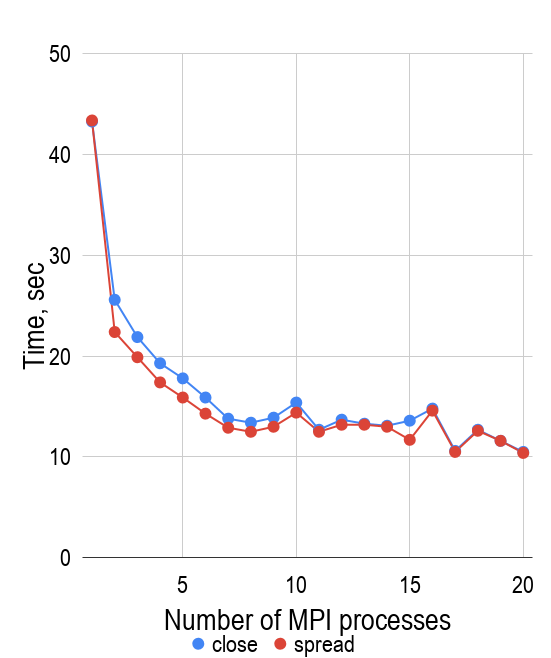
\includegraphics[width=0.48\textwidth]{figures/chapter-2/spread-vs-close/grs-cluster/k3-18.png}} &
		\subfloat[HW2 - k3-18]{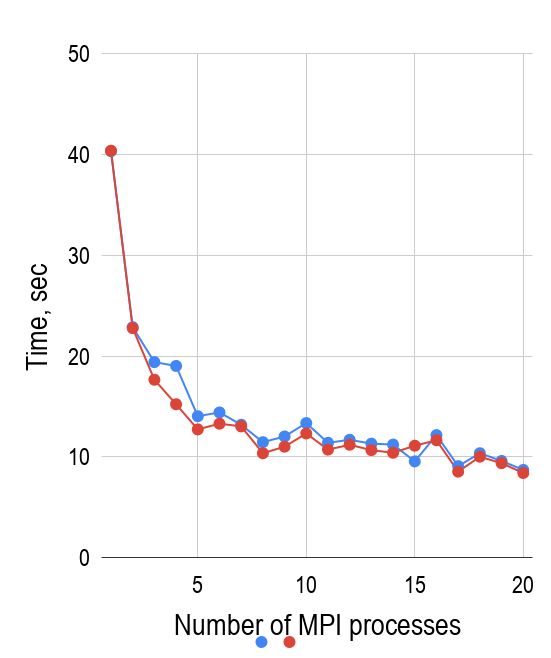
\includegraphics[width=0.48\textwidth]{figures/chapter-2/spread-vs-close/linux-cluster/k3-18.png}} \\
	\end{tabular}
	\caption{Comparison of \textit{close} and \textit{spread} pinning strategies}
	\label{fig:mumps-close-vs-spread-2}
\end{figure}




\figpointer{\ref{fig:mumps-close-vs-spread-3}}
\begin{figure}[htpb]
\centering
	\begin{tabular}{cc}
		\subfloat[HW1 - PFlow\_742]{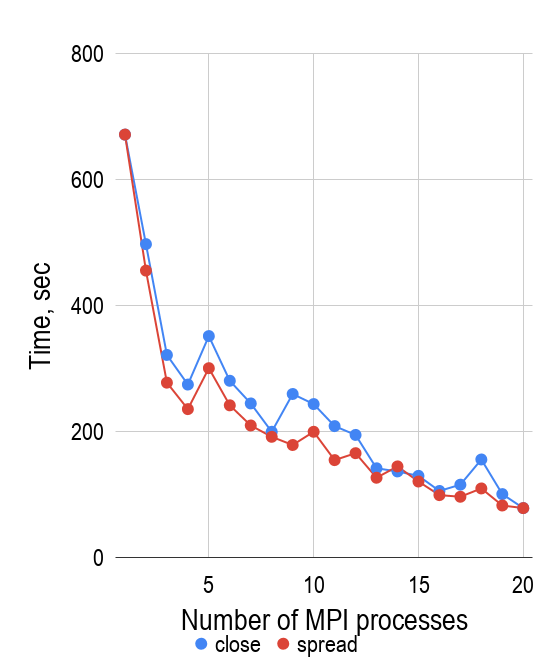
\includegraphics[width=0.48\textwidth]{figures/chapter-2/spread-vs-close/grs-cluster/PFlow_742.png}} &
		\subfloat[HW2 - PFlow\_742]{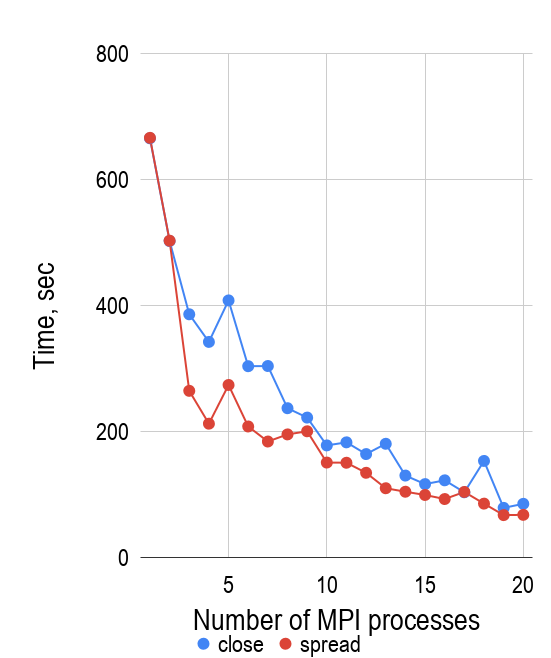
\includegraphics[width=0.48\textwidth]{figures/chapter-2/spread-vs-close/linux-cluster/PFlow_742.png}} \\
		\subfloat[HW1 - CurlCurl\_3]{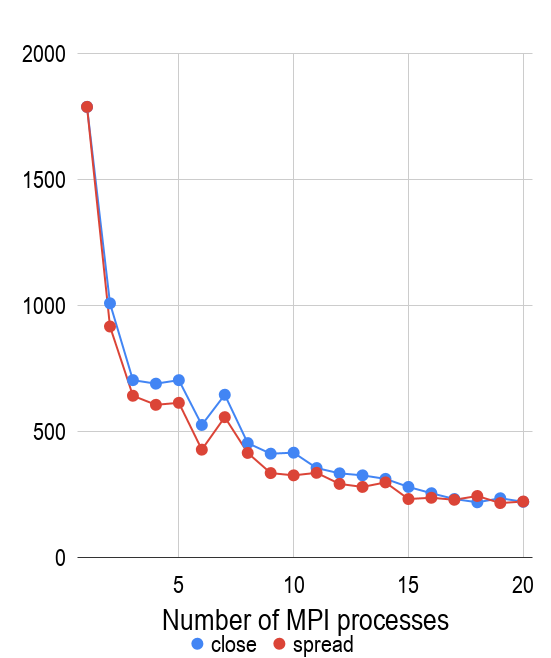
\includegraphics[width=0.48\textwidth]{figures/chapter-2/spread-vs-close/grs-cluster/CurlCurl_3.png}} &
		\subfloat[HW2 - CurlCurl\_3]{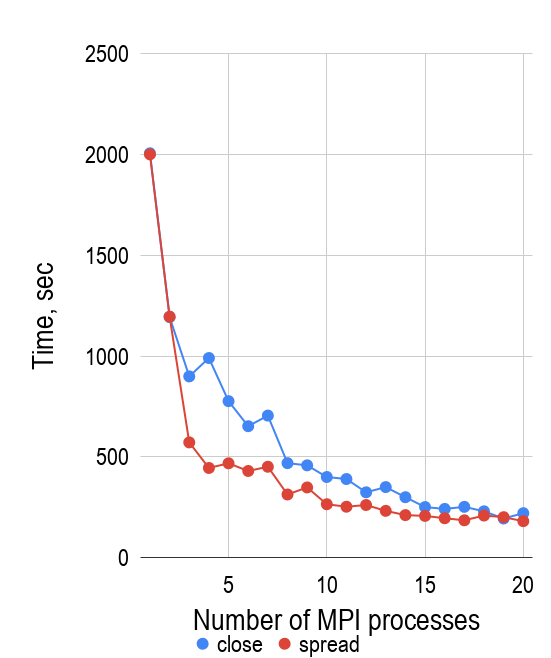
\includegraphics[width=0.48\textwidth]{figures/chapter-2/spread-vs-close/linux-cluster/CurlCurl_3.png}} \\
	\end{tabular}
	\caption{Comparison of \textit{close} and \textit{spread} pinning strategies}
	\label{fig:mumps-close-vs-spread-3}
\end{figure}


The tests revealed that, in the general case, \textit{spread}-pinning strategy performed better for both machines. On average, the strategy allows to reduce run-time by approximately \textbf{5.5\%} and \textbf{13.8\%} for HW1 and HW2 machines, respectively. The main performance gain can be observed in the middle range of the process count i.e. the range from 2 to 12 MPI processes, where  performance curves of \textit{spread} and \textit{close} strategies noticeably deviate. On the other hand, the difference becomes less and less prominent while the process count is reaching either its maximum or minimal values. In these cases, the difference between process distributions of both strategies becomes less noticeable as well. As an extreme example, the points where the process count is equal to 1 and 20 show the same performance, in case of HW1 machine which posses only 20 cores in a compute-node, because the points basically represent exactly the same process distributions.\\


It is also important to investigate performance gain around the saturation point i.e. the point after which a further increase of the process count results in either stagnation or drop of computer program speed-up. It is worth pointing out that from time to time it becomes very difficult to decide where the saturation point locates because of jagged behavior of speed-up curves. For this reason, a careful analysis of each performance graph was performed based on values of speed-up, efficiency and our subjective opinion. The results are summarized in tables \ref{table:pinning-comparison-grs-matrix-set} and \ref{table:pinning-comparison-suitesparse-matrix-set}. \\


\begin{table}[htpb]
\centering
\small
\begin{tabular}{c|c|c|c|c|c|c|c|c|c|}
\cline{2-5} \cline{7-10}
                                                                            & \multicolumn{4}{c|}{HW1}                                                                                                                                                                  &  & \multicolumn{4}{c|}{HW2}                                                                                                                                                                  \\ \cline{1-5} \cline{7-10} 
\multicolumn{1}{|c|}{\begin{tabular}[c]{@{}c@{}}Matrix\\ Name\end{tabular}} & MPI & \begin{tabular}[c]{@{}c@{}}Gain\\ w.r.t\\ "close", \\ \%\end{tabular} & \begin{tabular}[c]{@{}c@{}}Speed\\ up\end{tabular} & \begin{tabular}[c]{@{}c@{}}Effi-\\ ciency\end{tabular} &  & MPI & \begin{tabular}[c]{@{}c@{}}Gain\\ w.r.t\\ "close", \\ \%\end{tabular} & \begin{tabular}[c]{@{}c@{}}Speed\\ up\end{tabular} & \begin{tabular}[c]{@{}c@{}}Effi-\\ ciency\end{tabular} \\ \cline{1-5} \cline{7-10} 
\multicolumn{1}{|c|}{pwr-3d}                                                & 4   & 11.594                                                             & 1.386                                              & 0.347                                                  & \multicolumn{1}{c|}{} & 4   & 6.616                                                              & 1.626                                              & 0.406                                                  \\ \cline{1-5} \cline{7-10} 
\multicolumn{1}{|c|}{cube-5}                                                & 4   & 8.261                                                              & 1.139                                              & 0.285                                                  & \multicolumn{1}{c|}{} & 4   & 10.640                                                             & 1.156                                              & 0.289                                                  \\ \cline{1-5} \cline{7-10} 
\multicolumn{1}{|c|}{cube-64}                                               & 8   & 5.645                                                              & 1.812                                              & 0.226                                                  & \multicolumn{1}{c|}{} & 8   & 7.521                                                              & 1.729                                              & 0.216                                                  \\ \cline{1-5} \cline{7-10} 
\multicolumn{1}{|c|}{cube-645}                                              & 6   & 9.985                                                              & 2.152                                              & 0.359                                                  & \multicolumn{1}{c|}{} & 8   & 9.078                                                              & 2.521                                              & 0.315                                                  \\ \cline{1-5} \cline{7-10} 
\multicolumn{1}{|c|}{k3-2}                                                  & 7   & 7.788                                                              & 2.899                                              & 0.414                                                  & \multicolumn{1}{c|}{} & 8   & 9.947                                                              & 3.298                                              & 0.412                                                  \\ \cline{1-5} \cline{7-10} 
\multicolumn{1}{|c|}{k3-18}                                                 & 8   & 6.716                                                              & 3.472                                              & 0.434                                                  & \multicolumn{1}{c|}{} & 8   & 9.567                                                              & 3.896                                              & 0.487                                                  \\ \cline{1-5} \cline{7-10} 
\end{tabular}
\caption{Analysis and comparison of MUMPS performance at the saturation point between HW1 and HW2 for GRS matrix set}
\label{table:pinning-comparison-grs-matrix-set}
\end{table}



\begin{table}[htpb]
\centering
\small
\begin{tabular}{c|c|c|c|c|c|c|c|c|c|}
\cline{2-5} \cline{7-10}
                                                                            & \multicolumn{4}{c|}{HW1}                                                                                                                                                                  &  & \multicolumn{4}{c|}{HW2}                                                                                                                                                                  \\ \cline{1-5} \cline{7-10} 
\multicolumn{1}{|c|}{\begin{tabular}[c]{@{}c@{}}Matrix\\ Name\end{tabular}} & MPI & \begin{tabular}[c]{@{}c@{}}Gain\\ w.r.t\\ "close", \\ \%\end{tabular} & \begin{tabular}[c]{@{}c@{}}Speed\\ up\end{tabular} & \begin{tabular}[c]{@{}c@{}}Effi-\\ ciency\end{tabular} &  & MPI & \begin{tabular}[c]{@{}c@{}}Gain\\ w.r.t\\ "close", \\ \%\end{tabular} & \begin{tabular}[c]{@{}c@{}}Speed\\ up\end{tabular} & \begin{tabular}[c]{@{}c@{}}Effi-\\ ciency\end{tabular} \\ \cline{1-5} \cline{7-10} 
\multicolumn{1}{|c|}{cant}                                                  & 8   & 7.914                                                                 & 3.297                                              & 0.412                                                  &  & 8   & 12.437                                                                & 3.407                                              & 0.426                                                  \\ \cline{1-5} \cline{7-10} 
\multicolumn{1}{|c|}{consph}                                                & 15  & 0.110                                                                 & 6.147                                              & 0.410                                                  &  & 15  & 2.409                                                                 & 6.667                                              & 0.444                                                  \\ \cline{1-5} \cline{7-10} 
\multicolumn{1}{|c|}{CurlCurl\_3}                                           & 19  & 8.051                                                                 & 8.249                                              & 0.434                                                  &  & 20  & 17.908                                                                & 11.039                                             & 0.552                                                  \\ \cline{1-5} \cline{7-10} 
\multicolumn{1}{|c|}{Geo\_1438}                                             & 13  & 21.609                                                                & 4.548                                              & 0.350                                                  &  & ROM & ROM                                                                   & ROM                                                & ROM                                                    \\ \cline{1-5} \cline{7-10} 
\multicolumn{1}{|c|}{memchip}                                               & 9   & 11.290                                                                & 4.299                                              & 0.477                                                  &  & 9   & 11.102                                                                & 4.213                                              & 0.468                                                  \\ \cline{1-5} \cline{7-10} 
\multicolumn{1}{|c|}{PFlow\_742}                                            & 19  & 17.921                                                                & 8.106                                              & 0.427                                                  &  & 20  & 20.469                                                                & 9.798                                              & 0.490                                                  \\ \cline{1-5} \cline{7-10} 
\multicolumn{1}{|c|}{pkustk10}                                              & 17  & -0.664                                                                & 3.872                                              & 0.228                                                  &  & 17  & -1.108                                                                & 4.036                                              & 0.237                                                  \\ \cline{1-5} \cline{7-10} 
\multicolumn{1}{|c|}{torso3}                                                & 18  & 5.607                                                                 & 8.149                                              & 0.453                                                  &  & 19  & 6.028                                                                 & 9.493                                              & 0.499                                                  \\ \cline{1-5} \cline{7-10} 
\multicolumn{1}{|c|}{x104}                                                  & 6   & 9.537                                                                 & 1.789                                              & 0.298                                                  &  & 6   & 7.829                                                                 & 1.763                                              & 0.294                                                  \\ \cline{1-5} \cline{7-10} 
\end{tabular}
\caption{Analysis and comparison of MUMPS performance at the saturation point between HW1 and HW2 for SuiteSparse matrix set.\\
*ROM - run out of memory}
\label{table:pinning-comparison-suitesparse-matrix-set}
\end{table}


% comparison of different machines
A study of tables \ref{table:pinning-comparison-grs-matrix-set} and \ref{table:pinning-comparison-grs-matrix-set} reveals that HW2 machine performs slightly better in contrast to HW1 one with respect to parallel performance around the saturation points. This results are different from the overall performance gain mentioned above, however, they reflect the same trend. Additionally, it can be clearly observed that increase of NUMA domains always results in improving of efficiency and speed-up of MUMPS.\\

% Conclusion: process distribution can help in case of energy save computing

In this subsection, we have shown influence of different MPI process distributions and the number of NUMA domains on MUMPS parallel performance. We have observed that application of the \textit{spread} process distribution is always advantageous together with increase of the number of NUMA domains.\\ 


The result of this study can be relevant for energy-efficient parallel computing where a strong requirements to program efficiency are applied. This fact usually forces the user to reduce the process count and go away from the saturation point in order to keep values of efficiency around \textbf{0.7-0.8}. In this case, performance of MUMPS can be improved by \textbf{15-20\%} in contrast to a straightforward process pinning i.e. \textit{close} strategy.\\


Taken into account results of the tests, \textit{spread}-pinning has been chosen for the rest of the study. This process distribution can be easily achieved by means of some advanced OpenMPI command line options, for example \textit{--rank-by} and \textit{--bind-to}, as following:. \\

\begin{lstlisting}[language=bash, mathescape=false, caption={An example of \textit{spread}-pinning with using  advanced OpenMPI command line options}, frame=single, label={lst:iterative-refinement}]
mpiexec --rank-by numa --bind-to core -n $num_proc $executable_name $parameters
\end{lstlisting}
